\documentclass[fontscale=0.38,a0paper]{baposter}

\tracingstats=2

\usepackage{times}
\usepackage{calc}
\usepackage{graphicx}
\usepackage{amsmath}
\usepackage{amssymb}
\usepackage{relsize}
\usepackage{multirow}
\usepackage{bm}
\usepackage{caption}
\usepackage[authoryear,round]{natbib}
\usepackage[hidelinks]{hyperref}

\usepackage{tabularx}
\usepackage{booktabs}

\usepackage{colortbl}

\usepackage{multicol}

%\usepackage{pgfbaselayers}
%\pgfdeclarelayer{background}
%\pgfdeclarelayer{foreground}
%\pgfsetlayers{background,main,foreground}


% plr macros: these are for boxes in tables
\newcommand\tLL[1]{\multicolumn{1}{|c}{#1}}
\newcommand\tRR[1]{\multicolumn{1}{c|}{#1}}
\newcommand\tLR[1]{\multicolumn{1}{|c|}{#1}}
% nucleotides:
\newcommand{\nA}{\mbox{A}}  
\newcommand{\nC}{\mbox{C}}
\newcommand{\nG}{\mbox{G}}
\newcommand{\nT}{\mbox{T}}


%\usepackage{tikz}
%\usetikzlibrary{arrows,backgrounds,patterns,matrix,shapes,fit,calc,shadows,plotmarks,decorations.pathmorphing,positioning,trees}

\renewcommand{\familydefault}{\sfdefault}
\usepackage{helvet}
\usepackage{bookman}
\usepackage{palatino}

% My stuff
\newcommand{\E}{\mathbb{E}}
\renewcommand{\P}{\mathbb{P}}
% end my stuff

\selectcolormodel{cmyk}

% \graphicspath{{images/}}

%%%%%%%%%%%%%%%%%%%%%%%%%%%%%%%%%%%%%%%%%%%%%%%%%%%%%%%%%%%%%%%%%%%%%%%%%%%%%%%%
%%%% Some symbols used in the text
%%%%%%%%%%%%%%%%%%%%%%%%%%%%%%%%%%%%%%%%%%%%%%%%%%%%%%%%%%%%%%%%%%%%%%%%%%%%%%%%
%\newcommand{\sub}[2]{\ensuremath{#1_{\textrm{#2}}}}
%\newcommand{\gen}[2]{\ensuremath{\textrm{#1}_{\textrm{#2}}}}


%%%%%%%%%%%%%%%%%%%%%%%%%%%%%%%%%%%%%%%%%%%%%%%%%%%%%%%%%%%%%%%%%%%%%%%%%%%%%%%%
% Multicol Settings
%%%%%%%%%%%%%%%%%%%%%%%%%%%%%%%%%%%%%%%%%%%%%%%%%%%%%%%%%%%%%%%%%%%%%%%%%%%%%%%%
%\setlength{\columnsep}{0.7em}
\setlength{\columnsep}{8mm}
\setlength{\columnseprule}{0mm} % no vertical line


%%%%%%%%%%%%%%%%%%%%%%%%%%%%%%%%%%%%%%%%%%%%%%%%%%%%%%%%%%%%%%%%%%%%%%%%%%%%%%%%
% Save space in lists. Use this after the opening of the list
%%%%%%%%%%%%%%%%%%%%%%%%%%%%%%%%%%%%%%%%%%%%%%%%%%%%%%%%%%%%%%%%%%%%%%%%%%%%%%%%
\newcommand{\compresslist}{
\setlength{\itemsep}{1pt}
\setlength{\parskip}{0pt}
\setlength{\parsep}{0pt}
}

%%%%%%%%%%%%%%%%%%%%%%%%%%%%%%%%%%%%%%%%%%%%%%%%%%%%%%%%%%%%%%%%%%%%%%%%%%%%%%
%%% Other Macros
%%%%%%%%%%%%%%%%%%%%%%%%%%%%%%%%%%%%%%%%%%%%%%%%%%%%%%%%%%%%%%%%%%%%%%%%%%%%%%
% \renewcommand{\labelenumi}{\alph{enumi})}
% \renewcommand{\theenumi}{\alph{enumi})}
\newcommand{\postercaption}[1]{\begin{minipage}{\linewidth}\center\smaller
  {#1}\end{minipage}}



%%%%%%%%%%%%%%%%%%%%%%%%%%%%%%%%%%%%%%%%%%%%%%%%%%%%%%%%%%%%%%%%%%%%%%%%%%%%%%
%%% Begin of Document
%%%%%%%%%%%%%%%%%%%%%%%%%%%%%%%%%%%%%%%%%%%%%%%%%%%%%%%%%%%%%%%%%%%%%%%%%%%%%%

\begin{document}

%%%%%%%%%%%%%%%%%%%%%%%%%%%%%%%%%%%%%%%%%%%%%%%%%%%%%%%%%%%%%%%%%%%%%%%%%%%%%%
%%% Here starts the poster
%%%---------------------------------------------------------------------------
%%% Format it to your taste with the options
%%%%%%%%%%%%%%%%%%%%%%%%%%%%%%%%%%%%%%%%%%%%%%%%%%%%%%%%%%%%%%%%%%%%%%%%%%%%%%

% Define some colors
\definecolor{silver}{cmyk}{0,0,0,0.3}
\definecolor{black}{cmyk}{0,0,0.0,1.0}
\definecolor{white}{cmyk}{0,0,0.0,0.0}
\definecolor{darkSilver}{cmyk}{0,0,0,0.1}

\definecolor{darkYellow}{cmyk}{0,0,1.0,0.5}
\definecolor{yellow}{cmyk}{0,0,0.9,0.0}
\definecolor{reddishyellow}{cmyk}{0,0.22,1.0,0.0}
\definecolor{lightyellow}{cmyk}{0,0,0.3,0.0}
\definecolor{lighteryellow}{cmyk}{0,0,0.1,0.0}
\definecolor{lightestyellow}{cmyk}{0,0,0.05,0.0}

\definecolor{DavisBlue}{cmyk}{1,0.56,0,0.34}
%    C = 100  M = 56  Y = 0 K = 34


\definecolor{HohenheimBlue}{cmyk}{1,0.5,0,0.45}
\definecolor{HohenheimLightLightBlue}{RGB}{243,250,255}
\definecolor{HohenheimLightBlue}{RGB}{215,221,235}
\definecolor{HohenheimDarkBlue}{RGB}{52,104,152}
\definecolor{darkCyan}{cmyk}{1,1,0,0.5}
\definecolor{cyan}{cmyk}{1,0,0,0.0}
\definecolor{lightcyan}{cmyk}{0.3,0,0,0.0}
\definecolor{lightercyan}{cmyk}{0.1,0,0,0.0}
\definecolor{lightestcyan}{cmyk}{0.05,0,0,0.0}



\typeout{Poster Starts}
%Define custom background
\background{
  \begin{tikzpicture}[remember picture,overlay]%
    \draw (current page.north west)+(-2em,2em) node[anchor=north west] {\includegraphics[height=\textheight]{silhouettes_background}};
  \end{tikzpicture}%
}

\newlength{\leftimgwidth}
\begin{poster}%
  % Poster Options
  {
  % Columns and Column spacing
  columns=2,
  colspacing=1.5em,
  % Background
  % background=user,
  background=shade-tb,
  % Poster header options
  eyecatcher=yes,
  posterheaderheight=0.15\textheight,
  % Format of textbox header
  headerborder=open,
  % headershape=small-rounded,
  headershape=roundedright,
  headershade=shade-tb,
  % headershade=plain,
  headerfont=\Large\textsf, %Sans Serif
  % Format of textbox
  boxborder=small-rounded,
  % boxborder=roundedleft,    
  boxshade=plain,
  linewidth=0.5pt,
  % Color style
  % bgColorOne=lightestcyan,
  % bgColorTwo=lightcyan,
  bgColorOne=white,
  bgColorTwo=white,
  % borderColor=cyan,
  borderColor=black,
  headerColorOne=DavisBlue,
  % headerColorOne=cyan,
  headerColorTwo=black,
  % headerFontColor=black,
  headerFontColor=white,
  % boxColorOne=lightercyan,
  boxColorOne=HohenheimLightLightBlue,
  boxColorTwo=white,
  % Show grid to help with alignment
  grid=no
  % grid=yes
  }
  % Eye Catcher
  {
  \makebox[15em][r]{%
    \begin{minipage}{15em}
       \hfill
       
\includegraphics[width=15em]{USC-seal} \\
    \end{minipage}
    }
  }
  % Title
  {\sf %Sans Serif
  %\bf% %bold  
  \vspace{0.5em}
     \textbf{\textcolor{DavisBlue}{Local PCA finds heterogeneity in population structure along the genome}}\vspace{0.5em}}
  % Authors
  {\sf %Sans Serif
    Han Li$^{\dagger}$ and Peter Ralph$^{\dagger\ddagger}$ \\  \vspace{-1.0mm}
    {\small \textit{$\dagger$ Molecular \& Computational Biology, University of Southern California }}\\  
    {\small \textit{$\ddagger$ Mathematics and Biology, University of Oregon} }\\
    {\small   \url{http://biorxiv.org/content/early/2016/08/21/070615} }\\
    {\small   \url{https://github.com/petrelharp/local_pca} }\\
  }
  % Project logo
  {
    \makebox[15em][r]{%
      \begin{minipage}{15em}
        \hfill
          
\includegraphics[width=15em]{UOSignature-STK-BLK} \\
      \end{minipage}
    }
  }

  % Width of left inset image
%  \setlength{\leftimgwidth}{0.78em+0.0em}

%%%%%%%%%%%%%%%%%%%%%%%%%%%%%%%%%%%%%%%%%%%%%%%%%%%%%%%%%%%%%%%%%%%%%%%%%%%%%%
%%% Now define the boxes that make up the poster
%%%---------------------------------------------------------------------------
%%% Each box has a name and can be placed absolutely or relatively.
%%% The only inconvenience is that you can only specify a relative position 
%%% towards an already declared box. So if you have a box attached to the 
%%% bottom, one to the top and a third one which should be in between, you 
%%% have to specify the top and bottom boxes before you specify the middle 
%%% box.
%%%%%%%%%%%%%%%%%%%%%%%%%%%%%%%%%%%%%%%%%%%%%%%%%%%%%%%%%%%%%%%%%%%%%%%%%%%%%%

%%%%%%%%%%%%%%%%%%%%%%%%%%%%%%%%%%%%%%%%%%%%%%%%%%%%%%%%%%%%%%%%%%%%%%%%%%%%%%
\headerbox{What is local population structure?}{name=intro,column=0,row=0,span=1}{
%%%%%%%%%%%%%%%%%%%%%%%%%%%%%%%%%%%%%%%%%%%%%%%%%%%%%%%%%%%%%%%%%%%%%%%%%%%%%%

\emph{Population structure}: ``such matters as numbers, composition by age and sex, and state of subdivision'' \citep{wright1949genetical};
but also commonly, the genetic patterns that result from this process.
What aspects of demography should be included?  Should natural selection?
Incorporating differential survival or fecundity makes the concept less clear:
does a randomly mating population consisting of two types that are partially reproductively isolated from each other
have ``population structure''?

\emph{Whatever the definition},
selection causes the \emph{effects} of population structure --
\emph{realized} patterns of genetic relatedness --
to differ across the genome.
Locally adapted alleles are selected against in migrants,
increasing genetic differentiation between populations around this locus.
Or, newly adaptive alleles spread first in local populations.

We aim to describe 
how patterns of mean relatedness vary along the genome.
This works because:
geography establishes similar patterns of relatedness across much of the genome,
which are distorted locally by selection and other factors;
we look for commonalities in these distortions (\emph{not} outlier loci).


}
%%%%%%%%%%%%%%%%%%%%%%%%%%%%%%%%%%%%%%%%%%%%%%%%%%%%%%%%%%%%%%%%%%%%%%%%%%%%%%


%%%%%%%%%%%%%%%%%%%%%%%%%%%%%%%%%%%%%%%%%%%%%%%%%%%%%%%%%%%%%%%%%%%%%%%%%%%%%%
\headerbox{Our method}{name=method,column=0,span=1,below=intro}{
%%%%%%%%%%%%%%%%%%%%%%%%%%%%%%%%%%%%%%%%%%%%%%%%%%%%%%%%%%%%%%%%%%%%%%%%%%%%%%

    \begin{center}
    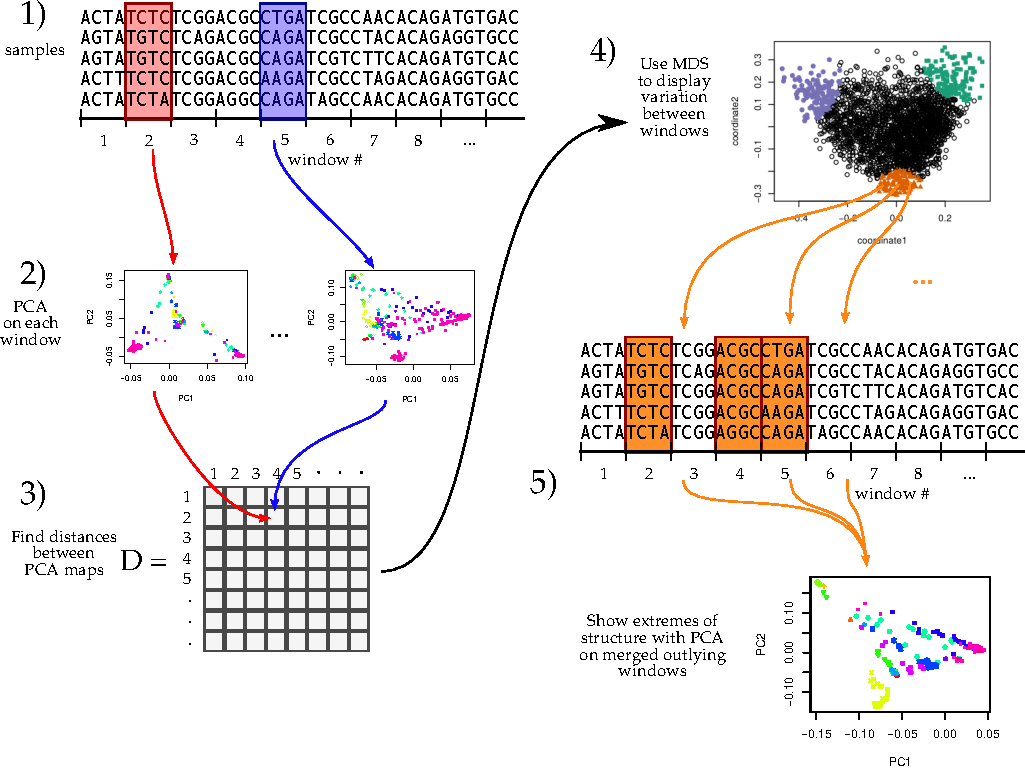
\includegraphics[width=\textwidth]{../the-method-diagram}
    \end{center}


    \begin{enumerate}
            \compresslist
        \item Code genome as $\{0,1,2\}$ and divide into windows (by \# SNPs, bp, or cM).
        \item Do PCA on each window: $\lambda^{(i)}_\ell$, $V^{(i)}_\ell$ the $\ell^\text{th}$ eigenvalue/vector of the covariance matrix for the $i^\text{th}$ window.
        \item Compute distances between windows:
            \[  
            D_{ij} = \| 
            \sum_{\ell=1}^k \frac{\lambda^{(i)}_\ell}{\sum_{m=1}^k\lambda^{(i)}_m} V^{(i)}_\ell (V^{(i)}_\ell)^T
            -
            \sum_{\ell=1}^k \frac{\lambda^{(j)}_\ell}{\sum_{m=1}^k\lambda^{(j)}_m} V^{(j)}_\ell (V^{(j)}_\ell)^T
            \|
            \]
        \item Visualize distances/similarities with MDS.
        \item Highlight similar regions of the genome.
        \item See how local PCA differs between regions by doing PCA after combining similar windows.
    \end{enumerate}

    \textbf{Notes:}
    \begin{enumerate}
            \compresslist
        \item Window size chosen by optimizing signal:noise \\
            (``signal:'' variance in PC scores across a chromosome; \\
            ``noise:'' average jackknife-estimated standard error of PC scores by window);\\
            in applications, hundreds to thousands per chromosome.
        \item Also used weighted PCA to remove the effects of oversampled groups without discarding data.
        \item Results insensitive to rough choice of window size or unit of measurement.
        \item Linear algebra reduced computation time of $D$ from weeks to seconds.
    \end{enumerate}

}
%%%%%%%%%%%%%%%%%%%%%%%%%%%%%%%%%%%%%%%%%%%%%%%%%%%%%%%%%%%%%%%%%%%%%%%%%%%%%%


%%%%%%%%%%%%%%%%%%%%%%%%%%%%%%%%%%%%%%%%%%%%%%%%%%%%%%%%%%%%%%%%%%%%%%%%%%%%%%
\headerbox{Results: \textit{Drosophila melanogaster}}{name=drosophila,column=1,row=0}{
%%%%%%%%%%%%%%%%%%%%%%%%%%%%%%%%%%%%%%%%%%%%%%%%%%%%%%%%%%%%%%%%%%%%%%%%%%%%%%

    380 Pan-African samples from Drosophila Genome Nexus \citep{lack2015drosophila}, \url{http://www.johnpool.net/genomes.html}.

    \centering
    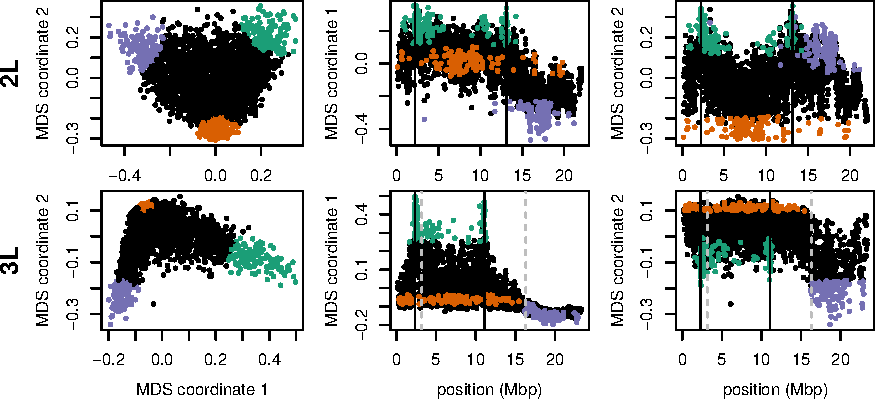
\includegraphics[width=\textwidth]{drosophila-MDS-extract}
    \postercaption{\textbf{Fig 1:}MDS, along the genome, for two chromosome arms.  Vertical lines corrspond to inversions.}

    \vspace{1em}

    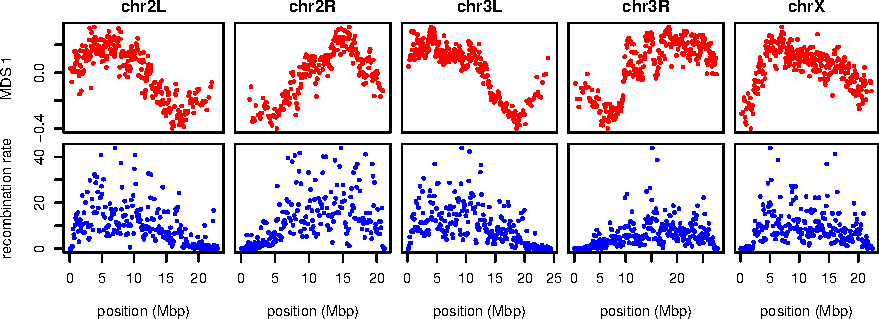
\includegraphics[width=\textwidth]{drosophila_just_recomb_mds}
    \postercaption{\textbf{Fig 2:}
        \emph{(top)} MDS, along the genome, \emph{after} removing inverted samples;\\
        \emph{(bottom)} recombination rate from \citep{fistonlavier2010drosophila}.
    }

}
%%%%%%%%%%%%%%%%%%%%%%%%%%%%%%%%%%%%%%%%%%%%%%%%%%%%%%%%%%%%%%%%%%%%%%%%%%%%%%


%%%%%%%%%%%%%%%%%%%%%%%%%%%%%%%%%%%%%%%%%%%%%%%%%%%%%%%%%%%%%%%%%%%%%%%%%%%%%%
\headerbox{Results: \textit{Homo sapiens}}{name=humans,column=1,below=drosophila}{
%%%%%%%%%%%%%%%%%%%%%%%%%%%%%%%%%%%%%%%%%%%%%%%%%%%%%%%%%%%%%%%%%%%%%%%%%%%%%%

    The POPRES dataset \citep{nelson2008population}:
    346 African-Americans, 73 Asians, 3,187 Europeans and 359 Indian Asians.
    (SNP array data; 500K markers)

    \centering
    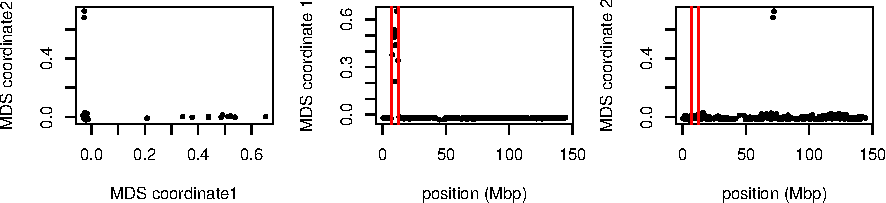
\includegraphics[width=\textwidth]{popres_chr8}
    \postercaption{\textbf{Fig 3:}
    MDS on chromosome 8. Vertical line is a large segregating inversion.}
  

}
%%%%%%%%%%%%%%%%%%%%%%%%%%%%%%%%%%%%%%%%%%%%%%%%%%%%%%%%%%%%%%%%%%%%%%%%%%%%%%


%%%%%%%%%%%%%%%%%%%%%%%%%%%%%%%%%%%%%%%%%%%%%%%%%%%%%%%%%%%%%%%%%%%%%%%%%%%%%%
\headerbox{Results: \textit{Medicago truncatula}}{name=medicago,column=1,below=humans}{
%%%%%%%%%%%%%%%%%%%%%%%%%%%%%%%%%%%%%%%%%%%%%%%%%%%%%%%%%%%%%%%%%%%%%%%%%%%%%%

    263 samples from 24 circum-Mediterranean countries,
    from the \textit{Medicago truncatula} Hapmap Project \citep{tang2014improved}.


    \centering

    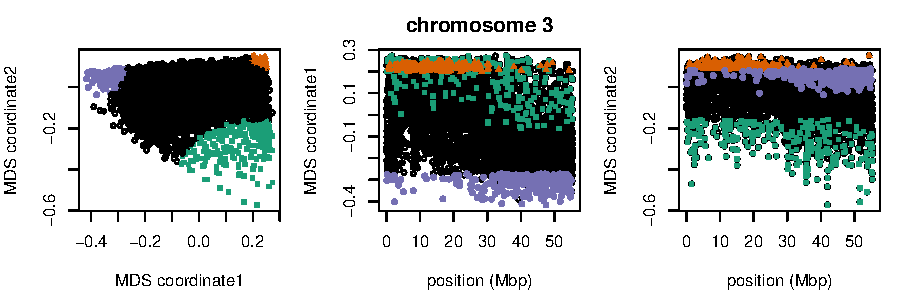
\includegraphics[width=0.8\textwidth]{../Fig6_Together_MDS_plot_chr3_final}
    \postercaption{\textbf{Fig 4:}
    MDS along chromosome 3, showing continuous variation.}
    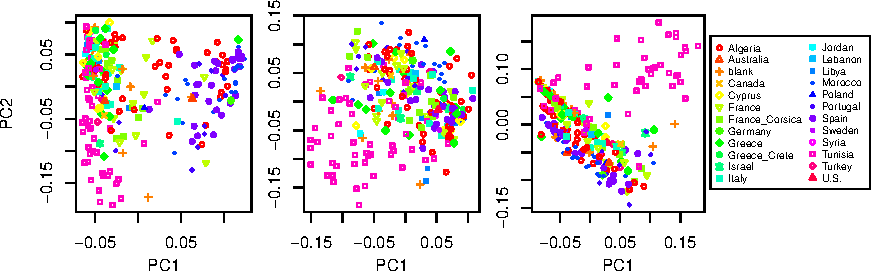
\includegraphics[width=0.8\textwidth]{medicago_PCA_chr3}
    \postercaption{\textbf{Fig 5:}
    PCA plots corresponding to windows in the three corners of the MDS triangle.}
    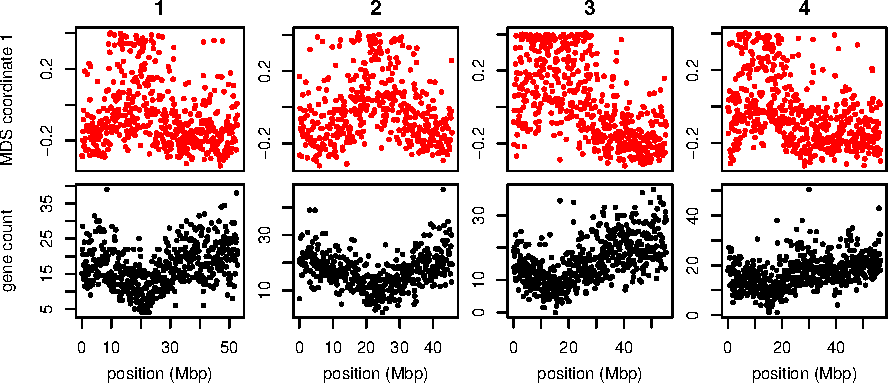
\includegraphics[width=0.7\textwidth]{medicago_mds_gene_count_extract}
    \postercaption{\textbf{Fig 6:}
    MDS score and local gene density along chromosomes 1--4.}


}
%%%%%%%%%%%%%%%%%%%%%%%%%%%%%%%%%%%%%%%%%%%%%%%%%%%%%%%%%%%%%%%%%%%%%%%%%%%%%%

%%%%%%%%%%%%%%%%%%%%%%%%%%%%%%%%%%%%%%%%%%%%%%%%%%%%%%%%%%%%%%%%%%%%%%%%%%%%%%
\headerbox{}{name=references,column=0,above=bottom}{
%%%%%%%%%%%%%%%%%%%%%%%%%%%%%%%%%%%%%%%%%%%%%%%%%%%%%%%%%%%%%%%%%%%%%%%%%%%%%%

    \textbf{Conclusion:}
    Variation mostly caused by segregating inversions
    and linked selection;
    how much varies by species.
    \vspace{1em}

    \textbf{R package:} available at \url{http://github.com/petrelharp/local_pca}\\
  \scriptsize
  \renewcommand{\section}[2]{\vskip 0.0em}
  \bibliographystyle{abbrvnat}
  \setlength{\bibsep}{0.0pt}
  \bibliography{../references}
  }
%%%%%%%%%%%%%%%%%%%%%%%%%%%%%%%%%%%%%%%%%%%%%%%%%%%%%%%%%%%%%%%%%%%%%%%%%%%%%%

\end{poster}%
\end{document}
